\begin{figure}[ht]
    \centering

    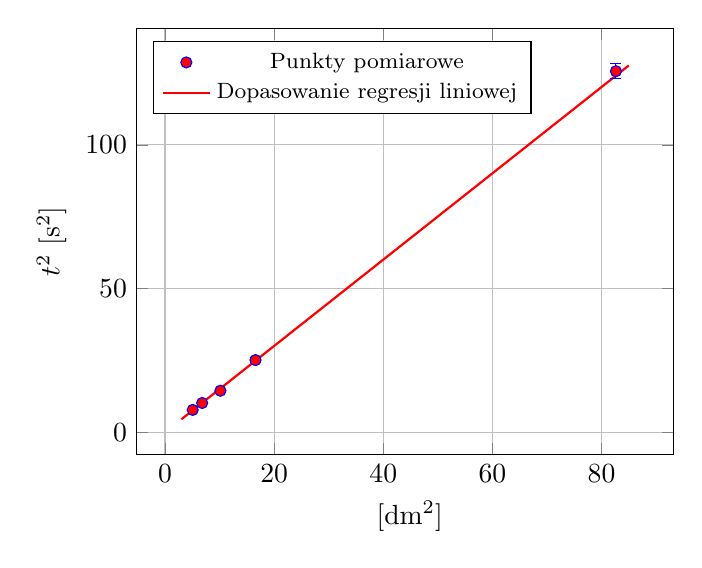
\begin{tikzpicture}
        \begin{axis}[
            width=8.4cm, height=7cm,
            xlabel={$\dwSq~[\mathrm{dm^2}]$},
            ylabel={$t^2~[\mathrm{s}^2]$},
            legend pos=north west,
            grid=major,
            legend style={font=\footnotesize}
        ]

        \addlegendimage{only marks, mark=*, blue, mark options={fill=red}, error bars/.cd, y dir=both, y explicit}
        \addlegendentry{Punkty pomiarowe}
        
        \addlegendimage{no markers, red, thick}
        \addlegendentry{Dopasowanie regresji liniowej}
        
        \def\slope{1.50007}
        \def\intercept{0.08968}
        
        \addplot [red, thick, domain=3:85, forget plot] {\slope*x + \intercept};
        \addlegendentry{Dopasowanie regresji liniowej}
    
        \addplot+[
            only marks,
            mark=*,
            blue,
            mark options={fill=red},
            forget plot,
            error bars/.cd,
            y dir=both,
            y explicit,
        ] table [x=x, y=y, y error=err] {
            x               y               err            
            10.15228426     14.52295881     0.4577332822   
            5.076142132     7.85456676      0.1789283481   
            82.6446281      125.6102978     2.581700008    
            16.58374793     25.17229584     0.7899873803   
            6.811989101     10.26817936     0.1653895391   
        };;
        \addlegendentry{Punkty pomiarowe}
    
        \end{axis}
    \end{tikzpicture}

    \caption{
        Dane pomiarowe dla Zależności III wraz z dopasowaniem regresji liniowej: $t^2(m^{-1}) = a~m^{-1} + b$. Niepewności $t^2$ są ledwo widoczne na wykresie, niepewności $m^{-1}$ są na tyle małe, że nie widać ich wcale.
    }
    \label{img:regresja-iii-wykres}
\end{figure}
